%%%%%%%%%%%%%%%%%%%%%%%%%%%%%%%
%%%%%%%%%%%%%%%%%%%%%%%%%%%%%%%
\chapter{Model structures}
%Basic understanding is introduced in this chapter.
\label{ch:models}
Parametric model structures for ship roll motion and manoeuvring are presented in this chapter. Model structures for roll are first introduced in \autoref{sec:roll}. 
The kinematics of the ship during manoeuvres is introduced in \autoref{sec:manoeuvring} with force models for the hull (\autoref{sec:hull}), rudders (\autoref{sec:rudders}), and propellers (\autoref{sec:propeller}).
\section{Roll motion} \label{sec:roll}
The roll motion without manoeuvres or external forces can be expressed by  \cite{himeno_prediction_1981},
\input{equations/roll_decay_equation_general_himeno}
\noindent where the static stability of the ship is expressed as the stiffness $C_{44}(\phi)$ with a function of the roll angle $\phi$, the damping $B_{44}(\dot{\phi})$ with a function of the roll velocity $\dot{\phi}$ and inertia $A_{44}$ connected to the roll acceleration $\ddot{\phi}$. The ship's roll motion can be observed under these conditions in a roll-decay test. The model is forced to an initial roll angle, as seen in \autoref{fig:rolldecay_initial}. The model is then released (\autoref{fig:rolldecay_free}) and rolls back to equilibrium (\autoref{fig:rolldecay_equilibrium}). The model will pass this static equilibrium point as a result of momentum and not stop until it has reached the end point on the other side (\autoref{fig:rolldecay_endpoint}). This motion starts a new cycle in which the model rolls back again. This new cycle results in oscillatory motion where potential energy is transferred to kinetic energy and back to potential energy.

\begin{figure}[H]
    \centering
    \begin{subfigure}[b,height=2cm]{0.22\textwidth}
         \centering
         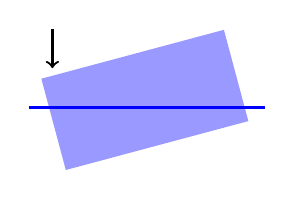
\begin{tikzpicture}

            \fill [blue!40, rotate around={15:(0,0.0)}] (-1.2,-0.5) rectangle (1.2,0.7);
            \draw[blue, thick] (-1.5,0) -- (1.5,0);
            \draw[black, thick, ->] (-1.2,1) -- (-1.2,0.5);
          
          \end{tikzpicture}
         \caption{The ship model is forces to an initial angle and then released}
         \label{fig:rolldecay_initial}
         \vspace{0.15cm}
     \end{subfigure}
     \hfill
     \begin{subfigure}[b,height=2cm]{0.22\textwidth}
         \centering
         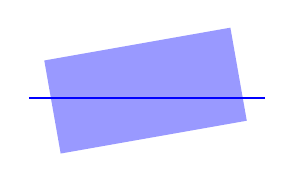
\begin{tikzpicture}

            \fill [blue!40, rotate around={10:(0,0.0)}] (-1.2,-0.5) rectangle (1.2,0.7);
            \draw[blue, thick] (-1.5,0) -- (1.5,0);
            
          \end{tikzpicture}
         \caption{Starts to roll back}
         \label{fig:rolldecay_free}
         \vspace{0.63cm}
     \end{subfigure}
     \hfill
     \begin{subfigure}[b,height=2cm]{0.22\textwidth}
         \centering
         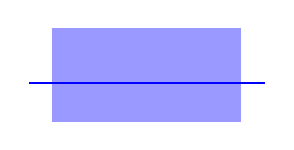
\begin{tikzpicture}

            \fill [blue!40, rotate around={0:(0,0.0)}] (-1.2,-0.5) rectangle (1.2,0.7);
            \draw[blue, thick] (-1.5,0) -- (1.5,0);
            
          \end{tikzpicture}
         \caption{Static water line.}
         \label{fig:rolldecay_equilibrium}
         \vspace{0.64cm}
     \end{subfigure}
    \hfill
     \begin{subfigure}[b,height=2cm]{0.22\textwidth}
         \centering
         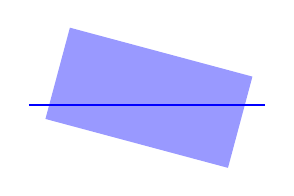
\begin{tikzpicture}

            \fill [blue!40, rotate around={-15:(0,0.0)}] (-1.2,-0.5) rectangle (1.2,0.7);
            \draw[blue, thick] (-1.5,0) -- (1.5,0);
            
          \end{tikzpicture}
         \caption{End point other side}
         \label{fig:rolldecay_endpoint}
         \vspace{0.36cm}
     \end{subfigure}
    \caption{Roll decay test.}
    \label{fig:rolldecay_procedure}
\end{figure}
\noindent This oscillation would never end if it was not for the roll damping. Interactions between the ship and the water, such as friction, wave generation, eddy generation, and hydrodynamic lift, will cause the ship to lose some of its energy. The energy loss means that the oscillation is decaying over time, as seen in \autoref{fig:rolldecay}, which displays the time series for the roll angle.

\begin{figure}[H]
    \centering
    \includegraphics[width=0.7\linewidth]{kappa/images/rolldecay_example.pdf}
    \caption{Example roll decay signal.}
    \label{fig:rolldecay}
\end{figure}

\noindent The damping $B_{44}\left(\dot{\phi}\right)$ can be expressed as an expansion series:  
\begin{equation}
    B_{44}\left(\dot{\phi}\right) = B_1\cdot\dot{\phi} + B_2\cdot\dot{\phi}\left|\dot{\phi}\right| + B_3\cdot\dot{\phi}^3 + ... + B_n\cdot\dot{\phi}^n
\end{equation}
 
\noindent This series can be truncated to be expressed as a ``linear model'' (\autoref{eq:roll_decay_equation_himeno_linear}), \say{quadratic model} (\autoref{eq:roll_decay_equation_himeno_quadratic_b}), and ``cubic model'' (\autoref{eq:roll_decay_equation_cubic}).
\input{equations/roll_decay_equation_himeno_linear}
\input{equations/roll_decay_equation_himeno_quadratic_b}
\input{equations/roll_decay_equation_cubic}
\subsection{Semi-empirical roll damping with Ikeda's method}
\label{sec:ikeda}
Ikeda's method \cite{ikeda_components_1978} divides roll damping into five damping components: the friction component $B_F$, the eddy component $B_E$, the lift component $B_L$, the wave component $B_W$, and the bilge keel component $B_{BK}$, as in the following Eq.(\ref{eq:ikeda}), 
\begin{equation} \label{eq:ikeda}
B_{44} = B_F + B_E + B_L + B_W + B_{BK}
\end{equation}
where the wave and eddy components require strip-theory based hydrodynamic analysis to obtain the ship's shape coefficients.
\subsection{Prime system} \label{sec:prime_system}
Some variables in the equations in this paper are expressed using nondimensional units with the prime system, denoted by the prime symbol ($'$). Variables are converted from SI units to the prime system using the denominators in \autoref{tab:prime_system} for the corresponding physical quantity, where $U$ and $L$ are the velocity and length between the perpendiculars of the ship, respectively, and $\rho$ is the water density.
For the calculation of surge velocity $u'$, the perturbed velocity $(u-U_0)$ about a nominal speed $U_0$ is used, as in \autoref{eq:u_prime}, to avoid a $u'$ of 1 for all speeds when the ship is on a straight course (where $u=U$), as in a resistance or self-propulsion test. The usage of the perturbed velocity, therefore, allows for higher order resistance terms in the model, such as $X_{u}$, which are otherwise not possible. 
\begin{equation}
    \label{eq:u_prime}
    u' = \frac{u-U_0}{U}
\end{equation}
For a nondimensional model, $U_0$ is instead expressed as a Froude number within the model (\autoref{eq:Fn0}), and this paper uses $F_{n0}=0.02$.
\begin{equation}
    \label{eq:Fn0}
    F_{n0} = \frac{U_0}{\sqrt{g \cdot L}}
\end{equation}
\begin{table}[h]
    \centering
    \caption{Scalings with prime system.}
    \label{tab:prime_system}
    \pgfplotstabletypeset[col sep=comma,
        columns={Physical quantity,SI unit,Denominator},
        columns/SI unit/.style={string type},
        columns/Physical quantity/.style={string type},
        columns/Denominator/.style={string type},
        column type=l,	% specify the align method
        every head row/.style={before row=\hline,after row=\hline},	% style the first row
        every last row/.style={after row=\hline},	% style the last row
    ]{tables/prime_system.prime_system.csv"}
\end{table}
\section{Manoeuvring} \label{sec:manoeuvring}
The ship manoeuvring dynamics is modeled as a state space model (\autoref{eq:state_space})
\begin{equation}
    \dot{\mathbf{x}}=f(\mathbf{x},\mathbf{u}) + q(t)
    \label{eq:state_space}
\end{equation}
where the change of state $\dot{\mathbf{x}}$ is expressed as function of the current state vector $\mathbf{x}$ and the input vector $\mathbf{u}$ through the transition function $f(\mathbf{x},\mathbf{u})$ and the process noise $q(t)$.  Process noise is considered when the model is used for filtering. However,  during deterministic simulations, it is usually set to zero $q(t)=0$.
A state with position and orientation, velocities, and turning rate defines the state of the ship in three degrees of freedom (\autoref{eq:state}). 
\begin{equation}
    \mathbf{x} = [x_0,y_0,\Psi, u,v,r]^T
    \label{eq:state}
\end{equation}
The ship’s kinematics are expressed amidship in a ship fixed reference frame, rotated around the Earth fixed axis $x_0$ by the heading angle $\Psi$ (\autoref{fig:reference_frames}). Forces and motions are expressed in the surge $X$, sway $Y$, and yaw $N$ degrees of freedom. The kinematics can be expressed as function of a velocity vector $\pmb{\bm{\upsilon}}$ (\autoref{eq:upsilon}), since the forces do not depend on the position ($x_0,y_0$) or heading $\Psi$, during the manoeuvre.
\begin{equation}
    \label{eq:upsilon}
    %\mathbf{\upsilon} = \left[\begin{matrix}u\\v\\r\end{matrix}\right]
    \pmb{\bm{\upsilon}} = \left[\begin{matrix}u\\v\\r\end{matrix}\right]
\end{equation}
The equation of motion can thus be expressed as \autoref{eq:eom}
\begin{equation}
    \label{eq:eom}
    \mathbf{F} = \mathbf{M}  \pmb{\bm{\dot{\upsilon}}} 
\end{equation}
where $\pmb{\bm{\dot{\upsilon}}}$ is the acceleration vector, $\mathbf{M}$ is the system inertia matrix and $\mathbf{F}$ is the total force vector.
The velocity transition can thus be expressed as
\begin{equation}
    \label{eq:acc}
    \pmb{\bm{\dot{\upsilon}}} = \mathbf{M}^{-1}\mathbf{F}
\end{equation}
\begin{figure}[h]
    \centering
    \includesvg{figures/reference_frames.svg}
    \caption{Relations between the earth fixed and ship fixed reference frames, showing the velocities and forced in the ship fixed frame.}
    \label{fig:reference_frames}
\end{figure}

The total forces can be divided into the Coriolis–centripetal matrix $\mathbf{C}$ and the damping force vector $\mathbf{D}$ \cite{fossenHandbookMarineCraft2011}. The control forces from the rudder and propeller are included in the $\mathbf{D}$ matrix.
\begin{equation}
    \label{eq:upsilon1d}
\mathbf{F} = - \mathbf{C} \upsilon + \mathbf{D}
\end{equation}
$\mathbf{M}$ and $\mathbf{C}$ are calculated according to \textcite{fossenHandbookMarineCraft2011} as shown in \autoref{eq:M_expanded} and \autoref{eq:C_expanded}. 
\begin{equation}
    \label{eq:M_expanded}
    \mathbf{M} = \left[\begin{matrix}- X_{\dot{u}} + m & 0 & 0\\0 & - Y_{\dot{v}} + m & - Y_{\dot{r}} + m x_{G}\\0 & - N_{\dot{v}} + m x_{G} & I_{z} - N_{\dot{r}}\end{matrix}\right]
\end{equation}
\begin{equation}
    \label{eq:C_expanded}
    \mathbf{C} = \left[\begin{matrix}0 & - m r & Y_{\dot{r}} r + Y_{\dot{v}} v - m r x_{G}\\m r & 0 & - X_{\dot{u}} u\\- Y_{\dot{r}} r - Y_{\dot{v}} v + m r x_{G} & X_{\dot{u}} u & 0\end{matrix}\right]
\end{equation}
where the added masses $X_{\dot{u}},Y_{\dot{v}},Y_{\dot{r}},N_{\dot{v}},N_{\dot{r}} < 0$. 

If we introduce the damping forces vector:
\begin{equation}
    \label{eq:D}
    \mathbf{D} = \left[\begin{matrix}X_{D}\\Y_{D}\\N_{D}\end{matrix}\right]
\end{equation}
the total force vector $\mathbf{F}$ can now be expressed as:
\begin{equation}
    \label{eq:F_expanded}
    %F = \mathbf{D} + \mathbf{\tau_{wave}} + \mathbf{\tau_{wind}} + \mathbf{\tau} + \left[\begin{matrix}m r v - r \left(Y_{\dot{r}} r + Y_{\dot{v}} v - m r x_{G}\right)\\X_{\dot{u}} r u - m r u\\- X_{\dot{u}} u v - u \left(- Y_{\dot{r}} r - Y_{\dot{v}} v + m r x_{G}\right)\end{matrix}\right]
\mathbf{F} = 
\left[\begin{matrix}
X \\
Y \\
N \\
\end{matrix}\right]
=
\left[\begin{matrix}X_{D} - Y_{\dot{r}} r^{2} + m r^{2} x_{G} + r v \left(- Y_{\dot{v}} + m\right)\\Y_{D} + r u \left(X_{\dot{u}} - m\right)\\N_{D} + r u \left(Y_{\dot{r}} - m x_{G}\right) + \underbrace{u v \left(- X_{\dot{u}} + Y_{\dot{v}}\right)}_{\text{Munk moment}} \end{matrix}\right]
\end{equation}
\mynote{The yawing moment $N$ has the so called Munk moment \cite{fossenHandbookMarineCraft2011}:
$$
u v \left(- X_{\dot{u}} + Y_{\dot{v}}\right)
$$
In many other manoeuvring models such as the Abkowitz \cite{abkowitzShipHydrodynamicsSteering1964} or MMG model \cite{yasukawaIntroductionMMGStandard2015}, the Munk moment is not explicitly included in the equations. The Munk moment contribution will instead be included in some of the hull coefficients, typically $N_V$ or ideally $N_{uv}$ if such a coefficient exist in the model.}
\newline
\vspace{0.3cm}
\mynote{The sway force $Y$ has the apparent centrifugal force from added mass and rigid body mass: 
$$r u \left(X_{\dot{u}} - m\right)$$ where $X_{\dot{u}}<0$ so that both added mass and rigid body mass create the centrifugal force acting outward in the turn. Both the added mass and rigid body mass will thus act to starboard on a port turn.}

For the calculation of acceleration \autoref{eq:acc}, the inverse of the mass matrix $\mathbf{M}$ can be calculated as:
\begin{equation}
    \label{eq:M_inv}
    \mathbf{M}^{-1} = \left[\begin{matrix}\frac{1}{- X_{\dot{u}} + m} & 0 & 0\\0 & \frac{- I_{z} + N_{\dot{r}}}{S} & \frac{- Y_{\dot{r}} + m x_{G}}{S}\\0 & \frac{- N_{\dot{v}} + m x_{G}}{S} & \frac{Y_{\dot{v}} - m}{S}\end{matrix}\right]
\end{equation}
with the helper variable $S$ which can be calculated according to \autoref{eq:S}. 
\begin{equation}
    \label{eq:S}
    S = I_{z} Y_{\dot{v}} - I_{z} m - N_{\dot{r}} Y_{\dot{v}} + N_{\dot{r}} m + N_{\dot{v}} Y_{\dot{r}} - N_{\dot{v}} m x_{G} - Y_{\dot{r}} m x_{G} + m^{2} x_{G}^{2}
\end{equation}
$S=0$ would however mean that the mass matrix would not be invertible. The sign of each component in \autoref{eq:S} is shown in \autoref{eq:S_sign}.  
\begin{equation}
    \label{eq:S_sign}
    S = - \left|{I_{z} Y_{\dot{v}}}\right| - \left|{I_{z} m}\right| - \left|{N_{\dot{r}} Y_{\dot{v}}}\right| - \left|{N_{\dot{r}} m}\right| + \left|{N_{\dot{v}} Y_{\dot{r}}}\right| + \left|{m^{2} x_{G}^{2}}\right| + \left|{N_{\dot{v}} m x_{G}}\right| + \left|{Y_{\dot{r}} m x_{G}}\right|
\end{equation}
The magnitude of these components for a typical ship is expressed in a non-dimensional form in \autoref{tab:S}. The negative components are much larger than the positive ones, so $S$ will be nonzero and the mass matrix of a ship is thus always invertible.      
\begin{table}[h]
    \centering
    \small
    \caption{Signs and magnitudes of the components within helper variable $S$ for a typical ship in non-dimensional form.}
    \label{tab:S}
    \pgfplotstabletypeset[col sep=comma, column type=c, 
        columns/part/.style={column type=r,string type},
        columns/magnitude/.style={column type=r,string type, column name=magnitude},
        every head row/.style={before row=\hline,after row=\hline},
        every last row/.style={after row=\hline}
    ]{tables/155.10_Fossen_model.determinant.csv}
\end{table}
\FloatBarrier

\section{Hull model} \label{sec:hull}
The hull forces are expressed with the following general polynomials, which are expressed in prime system units (see \autoref{sec:prime_system}). The perturbed surge velocity allows for the extra resistance term ${X_u}'$, so the resistance curve does not need to be quadratic like in the MMG model.  
\begin{equation}
    \label{eq:X_H}
    {X_H'} = {X_{0}'} + {X_{rr}'} {r'}^{2} + {X_{u}'} {u'} + {X_{vr}'} {r'} {v'} + {X_{vv}'} {v'}^{2}
\end{equation}
%
\begin{equation}
    \label{eq:Y_H}
    {Y_H'} = {Y_{0}'} + {Y_{rrr}'} {r'}^{3} + {Y_{r}'} {r'} + {Y_{vrr}'} {r'}^{2} {v'} + {Y_{vvr}'} {r'} {v'}^{2} + {Y_{vvv}'} {v'}^{3} + {Y_{v}'} {v'}
\end{equation}
%
\begin{equation}
    \label{eq:N_H}
    {N_H'} = {N_{0}'} + {N_{rrr}'} {r'}^{3} + {N_{r}'} {r'} + {N_{vrr}'} {r'}^{2} {v'} + {N_{vvr}'} {r'} {v'}^{2} + {N_{vvv}'} {v'}^{3} + {N_{v}'} {v'}
\end{equation}
\section{Rudder models} \label{sec:rudders}
It has become evident during this investigation that having an accurate rudder model is very important to obtain good accuracy of the total manoeuvring model. Polynomial rudder models were used in Paper \ref{pap:pit}, which can well describe the rudder forces if a sufficient degree of polynomials is used. However, these models introduce a lot of multicollinearity to the model (see \autoref{sec:multicollinearity}) which is a great problem in system identification with parameter estimation from inverse dynamics (see \autoref{sec:IDR}); It is basically hard to distinguish between forces generated by the hull and the rudder when only the total force acting on the ship can be observed. Instead of using a data-driven rudder model, a semi-empirical deterministic rudder model (see \autoref{sec:semi-empirical}) was therefore introduced in \ref{pap:physics}. The rudder forces were calculated on the basis of the rudder main particulars and preset coefficients from the literature.

A third rudder model was introduced in Paper \ref{pap:vct} as a modified version of the MMG rudder model \cite{yasukawa_introduction_2015}. This model was found to be easier to adopt when very rich information about the rudder forces was available from the VCT data.
\subsection{Semi-empirical rudder model} \label{sec:semi-empirical}
The semi-empirical rudder model was proposed in Paper \ref{pap:physics}  as is a lifting line model similar to \textcite{kjellberg_sailing_2023}, \textcite{matusiak_dynamics_2021}, and \textcite{hughes_tempest_2011} that is primarily based on the rudder wind tunnel tests conducted by \textcite{whicker_free-stream_1958}. The surge and sway forces are expressed as rudder lift $L_R$ and rudder drag $D_R$, which are projected on the ship through the rudder inflow angle $\alpha_f$ (see \autoref{eq:X_R_semiempirical}, \autoref{eq:Y_R_semiempirical}, and \autoref{fig:inflow}).
This angle is the sum of the initial inflow to the rudder at a straight course $\gamma_0$ and the inflow to the rudder $\gamma$ due to propeller-induced speed, drift angle, and yaw rate of the ship, as shown in \autoref{eq:gamma_semiempirical}.
%
\begin{figure}[h]
    \centering
    \includesvg[pretex=\centering\fontsize{10}{11}]{figures/rudder_flow.svg}
    \caption{Inflow to the rudder.}
    \label{fig:inflow}
\end{figure}
%
\begin{equation}
    \label{eq:X_R_semiempirical}
    X_{R} = - F_{N} \left(t_{R} - 1\right) \sin{\left(\delta \right)}
\end{equation}
%
\begin{equation}
    \label{eq:Y_R_semiempirical}
    Y_{R } = D_{R } \sin{\left(\alpha_{f } \right)} + L_{R } \cos{\left(\alpha_{f } \right)}
\end{equation}
%
\begin{equation}
    \label{eq:alpha_f_semiempirical}
    \alpha_{f } = \gamma_{0 } + \gamma_{}
\end{equation}
%
\begin{equation}
    \label{eq:gamma_semiempirical}
    \gamma_{} = \operatorname{atan}{\left(\frac{V_{R y }}{V_{R x C }} \right)}
\end{equation}

The transverse velocity at the rudder $V_{Ry}$ is calculated by multiplying the ship's yaw rate $r$ and transverse velocity $v$ by their flow straightening values $\kappa_{rtot}$ and $\kappa_{vtot}$ (\autoref{eq:V_R_y_semiempirical}). The flow straightening values have linear and nonlinear dependencies of the geometric inflow angle $\gamma_g$ (\autoref{eq:gamma_g_semiempirical}), as calculated in \autoref{eq:kappa_r_tot_semiempirical} with $\kappa_r,\kappa_{r \gamma g}$ and \autoref{eq:kappa_v_tot_semiempirical} with $\kappa_v,\kappa_{v \gamma g}$, respectively, so that the flow straightening may vary for different inflow angles, which is an enhancement of the MMG model.
The axial velocity at the rudder $V_{RxC}$, including the velocity of the propeller race, is presented in \autoref{sec:velocity_in_the_propeller_slip_stream}.
\begin{equation}
    \label{eq:V_R_y_semiempirical}
    V_{R y } = - \kappa_{r tot } r x_{R} - \kappa_{v tot } v
\end{equation}
%
\begin{equation}
    \label{eq:kappa_r_tot_semiempirical}
    \kappa_{r tot } = \kappa_{r} + \kappa_{r \gamma g} \left|{\gamma_{g }}\right|
\end{equation}
%
\begin{equation}
    \label{eq:kappa_v_tot_semiempirical}
    \kappa_{v tot } = \kappa_{v} + \kappa_{v \gamma g} \left|{\gamma_{g }}\right|
\end{equation}
%
\begin{equation}
    \label{eq:gamma_g_semiempirical}
    \gamma_{g } = \operatorname{atan}{\left(\frac{- r x_{R} - v}{V_{R x C }} \right)}
\end{equation}
The yawing moment is modeled as the sway force multiplied by the lever arm $x_R$, as in \autoref{eq:N_R_semiempirical}.
\begin{equation}
    \label{eq:N_R_semiempirical}
    N_{R} = Y_{R} x_{r}
\end{equation}
%
%
\subsubsection{Rudder lift}
\label{sec:rudder lift}
With inspiration from the work of \textcite{villa_numerical_2020}, the total rudder lift is calculated as the sum of the lift at the rudder areas that are covered by the propeller $L_{RC}$ and that at the uncovered area $L_{RU}$, as shown in \autoref{eq:L_R_semiempirical} and \autoref{fig:rudder_coverage}.
\begin{equation}
    \label{eq:L_R_semiempirical}
    L_{R } = L_{R C } + L_{R U }
\end{equation}
%
\begin{figure}[h]
    \centering
    \includesvg{figures/rudder_coverage.svg}
    \caption{Rudder areas covered and uncovered by the propeller.}
    \label{fig:rudder_coverage}
\end{figure}
%
The lift forces are calculated (\autoref{eq:L_R_U_semiempirical} and \autoref{eq:L_R_C_semiempirical}) with the lift coefficient $C_L$. These equations are essentially the same except that the lift at the covered part $L_{RC}$ is diminished by the factor $\lambda_R$ (\autoref{eq:lambda_R_semiempirical}) because of the limited radius of the propeller slipstream in the lateral direction \cite{brix_manoeuvring_1993} (See \autoref{sec:rudder_models} for further details).
\begin{equation}
    \label{eq:L_R_U_semiempirical}
    L_{R U } = \frac{A_{R U} C_{L } V_{R U }^{2} \rho}{2}
\end{equation}
%
\begin{equation}
    \label{eq:L_R_C_semiempirical}
    L_{R C } = \frac{A_{R C} C_{L } V_{R C }^{2} \lambda_{R } \rho}{2}
\end{equation}
The velocities of the uncovered $V_{RU}$ and covered $V_{RC}$ parts of the rudder are calculated according to \ref{sec:velocity_outside_the_propeller_slip_stream} and \ref{sec:velocity_in_the_propeller_slip_stream}.
For a nonstalling rudder, the lift coefficient $C_L$ is calculated according to \textcite{whicker_free-stream_1958} with the additional parameter $K_{gap}$ as shown in \autoref{eq:C_L_semiempirical}.
\begin{equation}
    \label{eq:C_L_semiempirical}
    C_{L } = K_{gap } \left(\alpha_{} \frac{\partial C_L}{\partial \alpha} + \frac{C_{DC} \alpha_{} \left|{\alpha_{}}\right|}{AR_{e }}\right)
\end{equation}
%
\begin{equation}
    \label{eq:alpha_semiempirical}
    \alpha_{} = \delta + \gamma_{0 } + \gamma_{}
\end{equation}
The effective aspect ratio $AR_e$ accounts for the mirror image effect when the rudder is flush with the hull, and it is typically assumed to be twice the geometric aspect ratio $AR_g$ (\autoref{eq:AR_e_semiempirical} and \autoref{eq:AR_g_semiempirical}) \cite{hughes_tempest_2011}.
However, The wPCC rudder is not flush with the hull, so a gap is created between the rudder and rudder horn at larger rudder angles, reducing the pressure difference between the high- and low-pressure sides in the upper part of the rudder. \textcite{matusiak_dynamics_2021} proposed that the gap effect can be modeled as a reduced aspect ratio. Instead, this paper opts for a more straightforward approach based on experience. A factor $K_{gap}$ is introduced, calculated according to \autoref{eq:lambda_gap_semiempirical}. The gap effect is only activated above a threshold rudder angle $\delta_{lim}$, and the strength of the gap effect is modeled by a factor $s$, as in \autoref{fig:gap}.
%
\begin{equation}
    \label{eq:AR_g_semiempirical}
    AR_{g } = \frac{b_{R}^{2}}{A_{R}}
\end{equation}
%
\begin{equation}
    \label{eq:AR_e_semiempirical}
    AR_{e } = 2 AR_{g }
\end{equation}
%
\begin{equation}
    \label{eq:lambda_gap_semiempirical}
    K_{gap} = \begin{cases} 1 & \text{for}\: \delta_{lim} > \left|{\delta}\right| \\s \left(- \delta_{lim} + \left|{\delta}\right|\right)^{2} + 1 & \text{otherwise} \end{cases}
\end{equation}
\begin{figure}[h]
    \centering
    \includesvg[width=0.5\columnwidth]{figures/gap_effect.gap.svg}
    \caption{Rudder lift is reduced by the gap between the rudder and rudder horn for larger rudder angles.}
    \label{fig:gap}
\end{figure}

The lift slope of the rudder $\frac{\partial C_L}{\partial \alpha}$ is calculated using \autoref{eq:dC_L_dalpha_semiempirical}, where $a_0$ is the section lift curve slope (\autoref{eq:a_0_semiempirical}) and $\Omega$ is the sweep angle of the quarter chord line \cite{lewis_principles_1989}.
\begin{equation}
    \label{eq:dC_L_dalpha_semiempirical}
    \frac{\partial C_L}{\partial \alpha} = \frac{AR_{e } a_{0 }}{\sqrt{\frac{AR_{e }^{2}}{\cos^{4}{\left(\Omega \right)}} + 4} \cos{\left(\Omega \right)} + 1.8}
\end{equation}
%
%
\begin{equation}
    \label{eq:a_0_semiempirical}
    a_{0 } = 1.8 \pi
\end{equation}
%
Additionally, a small nonlinear part to $C_L$ is modeled by the cross-flow drag coefficient $C_{DC}$, which is calculated for a rudder with squared tip using \autoref{eq:C_D_crossflow_semiempirical}, where the taper ratio $\lambda$ is the ratio between the chords at the tip and the root of the rudder (\autoref{eq:lambda__semiempirical}) \cite{hughes_tempest_2011}. 
\begin{equation}
    \label{eq:C_D_crossflow_semiempirical}
    C_{DC} = 1.6 \lambda^{} + 0.1
\end{equation}
%
\begin{equation}
    \label{eq:lambda__semiempirical}
    \lambda^{} = \frac{c_{t}}{c_{r}}
\end{equation}
%
%
\subsubsection{Rudder drag}
\label{sec:rudder_drag}
The total rudder drag $D_R$ is calculated as a sum of the contributions from the parts covered and uncovered by the propeller, as in \autoref{eq:D_R_semiempirical}.
\begin{equation}
    \label{eq:D_R_semiempirical}
    D_{R } = 0.5 \rho \left(A_{R C} C_{D C } V_{R C }^{2} + A_{R U} C_{D U } V_{R U }^{2}\right)
\end{equation}
The drag coefficients $C_{DC}$ and $C_{DU}$ are calculated with semi-empirical formulas according to \ref{sec:CD}.


\subsection{Modified quadratic MMG rudder model}
A modified quadratic MMG rudder model is proposed in Paper \ref{pap:vct}, with two enhancements to the original MMG rudder model \cite{yasukawaIntroductionMMGStandard2015}. The first enhancement is to add the rudder initial inflow angle $\gamma_0$ to the calculation of the effective inflow angle to the rudder $\alpha_R$, by replacing equation 21 in \textcite{yasukawaIntroductionMMGStandard2015} with the modified equation (\autoref{eq:alpha_R2}). This allows the rudder model to produce a side force in the straight ahead condition, due to unsymmetrical flow from the propeller. 
\begin{equation}
    \label{eq:alpha_R2}
    %\alpha_{R} = \delta + \gamma_{0} + \operatorname{atan}{\left(\frac{v_{R}}{u_{R}} \right)}
    \alpha_{R} = \delta + \underbrace{\gamma_{0}}_{\text{ proposed}} + \operatorname{atan}{\left(\frac{v_{R}}{u_{R}} \right)}
\end{equation}
The rudder transverse velocity $v_R$ is calculated as:
\begin{equation}
    \label{eq:gamma_R2}
    v_{R} = V \beta_{R} \gamma_{R}
\end{equation}
where $\beta_R$ is the effective inflow angle to the rudder as function of both the drift angle $\beta$ and yaw rate $r$:
\begin{equation}
    \label{eq:beta_R}
    \beta_{R} = \beta - \frac{l_{R} r}{V}
\end{equation}
where $l_R$ is a lever arm to the rudder that is treated as an experimental constant.
The other enhancement is to allow for a quadratic relationship between the flow straightening coefficient $\gamma_R$ and the effective inflow angle $\beta_R$, by introducing two new coefficients $\gamma_{R2neg}$, and $\gamma_{R2pos}$ as shown in:  
\begin{equation}
    \label{eq:gamma_R2}
    \gamma_{R} = \begin{cases} \overbrace{\gamma_{R2 neg} \left|{\beta_{R}}\right|}^{proposed} +   
    \gamma_{R neg} & \text{for}\: \beta_{R} \leq 0 \\\gamma_{R2 pos} \left| 
    {\beta_{R}}\right| + \gamma_{R pos} & \text{otherwise} \end{cases}
\end{equation}

\section{Propeller model} \label{sec:propeller}
The surge forces from the propeller are taken as the propeller thrust multiplied by a thrust deduction factor $t_{df}$:
\begin{equation}
    \label{eq:X_P}
    X_P = (1-t_{df})T
\end{equation}
The propeller thrust $T$ is taken as the measured thrust from VCT or FRMTs in this thesis to reduce the uncertainty associated with the complex interactions involving the propeller, rudder, and hull. The propeller also generates side forces, especially for yaw rates, which have a small stabilizing effect on the ship. This stabilizing propeller moment can be approximately 5\% of the rudder yawing moment, as shown in \autoref{fig:propeller_size_force}.
This effect is not explicitly modeled in this thesis, so that $Y_P=0$, $N_P=0$. Since the propeller side force is included in the VCT data, it is implicitly incorporated into the hull coefficients.
\begin{figure}[h]
    \centering
    \includesvg{figures/model_propeller_side_force.propeller_size_force.svg}
    %\caption{Typical yawing moments from rudder and propeller for various yaw rates.}

    \begin{minipage}[t]{5.25in}
    \caption{Typical yawing moments from rudder and propeller for various yaw rates.}
	\label{fig:propeller_size_force}
    \end{minipage}
        
\end{figure}

%\subsection{Multicollinearity and generalization of models} \label{sec:multicollinearity}
The drift effect of the hydrodynamic coefficients is inevitable in modeling of ship manoeuvring motions by using the system identification. The drifts of hydrodynamic coefficients result from the so-called multicollinearity, meaning that if the input variables of a regression model are firmly linearly dependent on each other, the regression results of their coefficients may be incorrect \cite{luo_parameter_2016}.
%\section{Vessel manoeuvring models} \label{sec:manoeuvring model}
\label{\detokenize{02.01_manoeuvring models:vessel-manoeuvring-models}}\label{\detokenize{02.01_manoeuvring models:vmm}}\label{\detokenize{02.01_manoeuvring models::doc}}
\vspace{-0.2cm}
Ship manoeuvring is a simplified case of seakeeping. The encountering waves have been removed, assuming calm water conditions. The manoeuvring motions have low frequencies so that added masses and other hydrodynamic derivatives can be assumed as constants  \cite{fossen_handbook_2011}. Three manoeuvring models are used in this thesis: 
\begin{itemize}
    \item Linear (LVMM) \cite{matusiak_dynamics_2021}
    \item Abkowitz (AVMM) \cite{abkowitz_ship_1964}
    \item Modified Abkowitz (MAVMM), which is proposed in Paper \ref{pap:pit}
\end{itemize}

\noindent\autoref{\detokenize{02.01_manoeuvring models:coordinate-system}} shows the reference frames used in the manoeuvring models where \(x_0\) and \(y_0\) and heading \(\Psi\) are the global position and orientation of a ship fix reference frame \(O(x,y,z)\) (or rather \(O(x,y)\) when heave is excluded) with origin at midship. \(u\), \(v\), \(r\), \(X\), \(Y\) and \(N\) are velocities and forces in the ship fix reference frame.



\begin{figure}[H]
    \centering
    \includegraphics[width=0.8\textwidth]{kappa/images/coordinate_system.PNG}
    \caption{Reference frames.}
    \label{\detokenize{02.01_manoeuvring models:coordinate-system}}
\end{figure}

The manoeuvring equation can be described as \cite{fossen_handbook_2011},
\begin{equation}\label{equation:02.01_manoeuvring models:eqqsystem}
\begin{split}\displaystyle \left[\begin{matrix}- X_{\dot{u}} + m & 0 & 0\\0 & - Y_{\dot{v}} + m & - Y_{\dot{r}} + m x_{G}\\0 & - N_{\dot{v}} + m x_{G} & I_{z} - N_{\dot{r}}\end{matrix}\right] \left[\begin{matrix}\dot{u}\\\dot{v}\\\dot{r}\end{matrix}\right] = \left[\begin{matrix}m r^{2} x_{G} + m r v + \operatorname{X_{D}}{\left(u,v,r,\delta,thrust \right)}\\- m r u + \operatorname{Y_{D}}{\left(u,v,r,\delta,thrust \right)}\\- m r u x_{G} + \operatorname{N_{D}}{\left(u,v,r,\delta,thrust \right)}\end{matrix}\right]\end{split}
\end{equation}

\noindent where the first matrix describes the inertia of the ship in the surge, sway and yaw directions. The inertia in air is represented by the mass $m$ and moment of inertia $I_z$. The added mass in water is represented by: $X_{\dot{u}}$, $Y_{\dot{v}}$, $Y_{\dot{r}}$, $N_{\dot{v}}$ and $N_{\dot{r}}$. The hydrodynamic forces from the ship hull and rudder are desribed in the functions $X_D()$, $Y_D()$ and $N_D()$. The accelerations ($\dot{u}$, $\dot{v}$ and $\dot{r}$) can be solved from this equation,
\begin{equation}\label{equation:02.01_manoeuvring models:eqacc}
\begin{split}\displaystyle \dot{\nu} = \left[\begin{matrix}\dot{u}\\\dot{v}\\\dot{r}\end{matrix}\right] = \left[\begin{matrix}\frac{1}{- X_{\dot{u}} + m} & 0 & 0\\0 & - \frac{- I_{z} + N_{\dot{r}}}{S} & - \frac{- Y_{\dot{r}} + m x_{G}}{S}\\0 & - \frac{- N_{\dot{v}} + m x_{G}}{S} & - \frac{Y_{\dot{v}} - m}{S}\end{matrix}\right] \left[\begin{matrix}m r^{2} x_{G} + m r v + \operatorname{X_{D}}{\left(u,v,r,\delta,thrust \right)}\\- m r u + \operatorname{Y_{D}}{\left(u,v,r,\delta,thrust \right)}\\- m r u x_{G} + \operatorname{N_{D}}{\left(u,v,r,\delta,thrust \right)}\end{matrix}\right]\end{split}
\end{equation}

where \(S\) is a helper variable:
\begin{equation}\label{equation:02.01_manoeuvring models:eq_S}
\begin{split}\displaystyle S = - I_{z} Y_{\dot{v}} + I_{z} m + N_{\dot{r}} Y_{\dot{v}} - N_{\dot{r}} m - N_{\dot{v}} Y_{\dot{r}} + N_{\dot{v}} m x_{G} + Y_{\dot{r}} m x_{G} - m^{2} x_{G}^{2}\end{split}
\end{equation}


\noindent A state space model for manoeuvring can now be defined with six states:
\begin{equation}\label{equation:02.01_manoeuvring models:eq_x}
\begin{split}\displaystyle \mathbf{x} = \left[\begin{matrix}x_{0}\\y_{0}\\\Psi\\u\\v\\r\end{matrix}\right]\end{split}
\end{equation}
\noindent where $x_0$, $y_0$ and $\Psi$ are the global coordinates and heading of the ship and $u$, $v$ and $r$ are the velocities as seen in \autoref{\detokenize{02.01_manoeuvring models:coordinate-system}}.
The time derivative of this state \(\dot{\mathbf{x}}\) can be defined by a state transition \(f(\mathbf{x},\mathbf{c})\) using geometrical relations
how global coordinates \(x_0\), \(y_0\) and \(\Psi\) depend on \(u\), \(v\), and \(r\) viz.,
\begin{equation}\label{equation:02.01_manoeuvring models:eqf}
\begin{split}\displaystyle \dot{\mathbf{x}} = f(\mathbf{x},\mathbf{c}) + \mathbf{w}
                                          = \left[\begin{matrix}\dot{x_0}\\ \dot{y_0} \\ \dot{\Psi} \\\dot{u}\\\dot{v}\\\dot{r}\end{matrix}\right] + \mathbf{w}
                                          = \left[\begin{matrix}u \cos{\left(\Psi \right)} - v \sin{\left(\Psi \right)}\\u \sin{\left(\Psi \right)} + v \cos{\left(\Psi \right)}\\r\\\dot{u}\\\dot{v}\\\dot{r}\end{matrix}\right] + \mathbf{w}\end{split}
\end{equation}

where \(\mathbf{c}\) is control inputs (rudder angle \(\delta\) and thrust); the last three derivatives: \(\dot{u}\), \(\dot{v}\), \(\dot{r}\) are calculated with \autoref{equation:02.01_manoeuvring models:eqacc}.
\(\mathbf{w}\) is the process noise, i.e., the difference between the predicted state by the manoeuvring model and the true
state of the system. \(\mathbf{w}\) is unknown when the manoeuvring model is used for manoeuvre predictions and therefore normally
assumed to be zero, but it is an important factor when the manoeuvring model is used in the EKF (see \autoref{sec:datacleaning}).
The manoeuvring simulation can now be conducted by numerical integration of \autoref{equation:02.01_manoeuvring models:eqf}. The main difference between the manoeuvring model:s lies in how the hydrodynamic functions \(X_D(u,v,r,\delta,thrust)\), \(Y_D(u,v,r,\delta,thrust)\), \(N_D(u,v,r,\delta,thrust)\) are defined. These expressions are denoted in prime system ($X_D'$, $Y_D'$, $N_D'$) below for the various manoeuvring models: LVMM, AVMM and MAVMM.

\subsubsection*{{\normalfont \textbf{Linear vessel manoeuvring model (LVMM) \cite{matusiak_dynamics_2021}}}}
\begin{equation}\label{equation:02.01_manoeuvring models:eqxlinear}
\begin{split}\begin{split}
\operatorname{X_{D}'}{\left(u',v',r',\delta\right)} = & X_{\delta} \delta + X_{r} r' + X_{u} u' + X_{v} v' 
\end{split}\end{split}
\end{equation}\begin{equation}\label{equation:02.01_manoeuvring models:eqylinear}
\begin{split}\begin{split}
\operatorname{Y_{D}'}{\left(u',v',r',\delta \right)} = & Y_{\delta} \delta + Y_{r} r' + Y_{u} u' + Y_{v} v' 
\end{split}\end{split}
\end{equation}\begin{equation}\label{equation:02.01_manoeuvring models:eqnlinear}
\begin{split}\begin{split}
\operatorname{N_{D}'}{\left(u',v',r',\delta \right)} = & N_{\delta} \delta + N_{r} r' + N_{u} u' + N_{v} v' 
\end{split}\end{split}
\end{equation}

\subsubsection*{\normalfont \textbf{Abkowitz vessel manoeuvring model (AVMM) \cite{abkowitz_ship_1964}}}
\begin{equation}\label{equation:02.01_manoeuvring models:eqxabkowitz}
\begin{split}
\operatorname{X_{D}'}{\left(u',v',r',\delta,thrust' \right)} = & X_{\delta\delta} \delta^{2} + X_{r\delta} \delta r' + X_{rr} r'^{2} + X_{T} thrust' + X_{u\delta\delta} \delta^{2} u' \\ 
& + X_{ur\delta} \delta r' u' + X_{urr} r'^{2} u' + X_{uuu} u'^{3} + X_{uu} u'^{2} \\ 
& + X_{uv\delta} \delta u' v' + X_{uvr} r' u' v' + X_{uvv} u' v'^{2} \\
& + X_{u} u' + X_{v\delta} \delta v' + X_{vr} r' v' + X_{vv} v'^{2} 
\end{split}
\end{equation}

\begin{equation}\label{equation:02.01_manoeuvring models:eqyabkowitz}
\begin{split}\begin{split}
\operatorname{Y_{D}'}{\left(u',v',r',\delta,thrust' \right)} = & Y_{0uu} u'^{2} + Y_{0u} u' + Y_{0} + Y_{\delta\delta\delta} \delta^{3} + Y_{\delta} \delta + Y_{r\delta\delta} \delta^{2} r' + Y_{rr\delta} \delta r'^{2} \\ & + Y_{rrr} r'^{3} + Y_{r} r' + Y_{T\delta} \delta thrust' + Y_{T} thrust' + Y_{u\delta} \delta u' \\ & + Y_{ur} r' u' + Y_{uu\delta} \delta u'^{2} + Y_{uur} r' u'^{2} + Y_{uuv} u'^{2} v' + Y_{uv} u' v' \\ & + Y_{v\delta\delta} \delta^{2} v' + Y_{vr\delta} \delta r' v' + Y_{vrr} r'^{2} v' + Y_{vv\delta} \delta v'^{2} + Y_{vvr} r' v'^{2} \\ & + Y_{vvv} v'^{3} + Y_{v} v' 
\end{split}\end{split}
\end{equation}\begin{equation}\label{equation:02.01_manoeuvring models:eqnabkowitz}
\begin{split}\begin{split}
\operatorname{N_{D}'}{\left(u',v',r',\delta,thrust' \right)} = & N_{0uu} u'^{2} + N_{0u} u' + N_{0} + N_{\delta\delta\delta} \delta^{3} + N_{\delta} \delta + N_{r\delta\delta} \delta^{2} r' + N_{rr\delta} \delta r'^{2} \\ & + N_{rrr} r'^{3} + N_{r} r' + N_{T\delta} \delta thrust' + N_{T} thrust' + N_{u\delta} \delta u' \\ & + N_{ur} r' u' + N_{uu\delta} \delta u'^{2} + N_{uur} r' u'^{2} + N_{uuv} u'^{2} v' + N_{uv} u' v' \\ & + N_{v\delta\delta} \delta^{2} v' + N_{vr\delta} \delta r' v' + N_{vrr} r'^{2} v' + N_{vv\delta} \delta v'^{2} + N_{vvr} r' v'^{2} \\ & + N_{vvv} v'^{3} + N_{v} v' 
\end{split}\end{split}
\end{equation}

\subsubsection*{\normalfont \textbf{Modified Abkowitz vessel manoeuvring model (MAVMM)}}
\newline
Only the most relevant coefficients in AVMM are included, as proposed in Paper \ref{pap:pit}.
\begin{equation}\label{equation:02.01_manoeuvring models:eqxmartinssimple}
\begin{split}\begin{split}
\operatorname{X_{D}'}{\left(u',v',r',\delta,thrust' \right)} = & X_{\delta\delta} \delta^{2} + X_{rr} r'^{2} + X_{T} thrust' + X_{uu} u'^{2} + X_{u} u' + X_{vr} r' v' 
\end{split}\end{split}
\end{equation}\begin{equation}\label{equation:02.01_manoeuvring models:eqymartinssimple}
\begin{split}\begin{split}
\operatorname{Y_{D}'}{\left(u',v',r',\delta,thrust' \right)} = & Y_{\delta} \delta + Y_{r} r' + Y_{T\delta} \delta thrust' + Y_{T} thrust' + Y_{ur} r' u' + Y_{u} u' \\ & + Y_{vv\delta} \delta v'^{2} + Y_{v} v' 
\end{split}\end{split}
\end{equation}\begin{equation}\label{equation:02.01_manoeuvring models:eqnmartinssimple}
\begin{split}\begin{split}
\operatorname{N_{D}'}{\left(u',v',r',\delta,thrust' \right)} = & N_{\delta} \delta + N_{r} r' + N_{T\delta} \delta thrust' + N_{T} thrust' + N_{ur} r' u' + N_{u} u' \\ & + N_{vv\delta} \delta v'^{2} + N_{v} v' 
\end{split}\end{split}
\end{equation}

The hydrodynamic functions above are expressed using nondimensional units with the prime system, denoted by the prime symbol (\('\)). The quantities are expressed in the prime system, using the denominators in \autoref{tab:prime-system-denominators}. For instance, surge linear velocity \(u\) can be expressed in the prime system as seen in \autoref{equation:02.01_manoeuvring models:eqprime} using the linear velocity denominator.
\begin{equation}\label{equation:02.01_manoeuvring models:eqprime}
\begin{split}\displaystyle u'=\frac{u}{V}\end{split}
\end{equation}

Equations can either be written in the Prime or regular Standard Institute (SI) system. The hydrodynamic derivatives are always expressing forces in the prime system as function of state variables. The (\('\)) sign is therefore implicit and not written out as seen in \autoref{equation:02.01_manoeuvring models:eqderivativeprime}.
\begin{equation}\label{equation:02.01_manoeuvring models:eqderivativeprime}
\begin{split}\displaystyle Y_{\delta'}'=\frac{\partial Y_D'}{\partial \delta'} := Y_{\delta} \end{split}
\end{equation}

The exceptions are the added masses (\(X_{\dot{u}}\), \(Y_{\dot{v}}\), \(Y_{\dot{r}}\), \(N_{\dot{v}}\) and \(N_{\dot{r}}\)) which are expressed in both Prime system or the regular SI system where the (\('\)) sign is therefore
explicitly stated.
There is however a great benefit in expressing the hydrodynamic forces in the prime system. The forces are often nonlinear due to a quadratic relation to the flow velocity, as seen in \autoref{equation:02.01_manoeuvring models:eqquadraticsi}.
\begin{equation}\label{equation:02.01_manoeuvring models:eqquadraticsi}
\begin{split}\displaystyle Y_{D}=Y_{\delta} \cdot \delta \cdot \frac{L^2V^2\rho}{2}\end{split}
\end{equation}
which becomes linear when expressed in the prime system as seen in \autoref{equation:02.01_manoeuvring models:eqquadraticprime}.
\begin{equation}\label{equation:02.01_manoeuvring models:eqquadraticprime}
\begin{split}\displaystyle Y_{D}'=Y_{\delta} \cdot \delta'\end{split}
\end{equation}
%\subsection{The propeller model}
\label{\detokenize{02.10_propeller_model:the-propeller-model}}\label{\detokenize{02.10_propeller_model::doc}}
\sphinxAtStartPar
A propeller model is developed based on Manoeuvring Modeling Group (MMG) model \cite{yasukawa_introduction_2015} where the thrust is expressed as:
\begin{equation}\label{equation:02.10_propeller_model:eqT}
\begin{split}\displaystyle thrust = D^{4} K_{T} n^{2} \rho\end{split}
\end{equation}
\sphinxAtStartPar
and the thrust coefficient \(K_T\) is modelled as a second order polynomial:
\begin{equation}\label{equation:02.10_propeller_model:eqkt}
\begin{split}\displaystyle K_{T} = J^{2} k_{2} + J k_{1} + k_{0}\end{split}
\end{equation}
\sphinxAtStartPar
The advance ratio \(J\) is calculated as:
\begin{equation}\label{equation:02.10_propeller_model:eqJ}
\begin{split}\displaystyle J = \frac{u \left(1 - w_{p}\right)}{D n}\end{split}
\end{equation}
\sphinxAtStartPar
where \(D\) is propeller diameter, \(n\) is propeller speed and \(w_p\) is the wake fraction at an oblique inflow to the propeller from the drift angle and the yaw rate. A semi\sphinxhyphen{}empirical formula for \(w_p\) is provided in the MMG model. As an alternative, a simple polynomial is proposed in \autoref{equation:02.10_propeller_model:eqpropellermodel}.
\begin{equation}\label{equation:02.10_propeller_model:eqpropellermodel}
\begin{split}\displaystyle w_{p} = C_{1} \delta + C_{2} \delta^{2} + C_{3} \beta_{p}^{2} + C_{4} u + w_{p0}\end{split}
\end{equation}
\sphinxAtStartPar
\(w_p\) is modeled as a function of rudder angle \(\delta\), to include wake influence from the rudder and ship speed \(u\), to include a speed dependency. The influence from drift angle \(\beta\) and yaw rate \(r\) is expressed by \(\beta_p\) in \autoref{equation:02.10_propeller_model:eqbetap}.
\begin{equation}\label{equation:02.10_propeller_model:eqbetap}
\begin{split}\beta_p=\beta - \frac{r}{V} \cdot x_p \end{split}
\end{equation}
where \(x_p\) is the propeller longitudinal position and \(w_{p0}\) is the regular Taylor wake fraction, applicable to straight ahead steaming with no rudder angle. Similar to the MMG propeller model, two sets of parameters \(C_1\)-\(C_4\) should be used in the propeller model depending on the sign of \(\beta_p\).